\begin{enumerate}[label=\thesubsection.\arabic*.,ref=\thesubsection.\theenumi]
\numberwithin{equation}{enumi}

\item We are given with a feedback voltage amplifier shown in \ref{fig:Voltage feedback amplifier}.We can neglect $r_{o}$ and given with $R_{1}+R_{2}>>R_{D}$.\\
(a)Find expressions for G and H hence amount of feedback.\\
(b)Noting that the feedback can be eliminated by removing $R_{1}$ and $R_{2}$ and connecting the gate of Q to a constant dc voltage (signal ground) give the input resistance $R_{i}$ and output resistance $R_{o}$ of the open-amplifier.\\
(c)Using standard circuit analysis (i.e =, without invoking the feedback approach), find the input resistance $R_{if}$ and the output resistance $R_{of}$ .How does $R_{if}$ relate to $R_{i}$ and $R_{of}$ relates to $R_{o}$ ?\\


\begin{figure}[h!]
	\begin{center}
		\resizebox{\columnwidth/1}{!}{
 \begin{circuitikz}[american resistors]
  
  \ctikzset{bipoles/length=1cm}
  
  \draw[color=black]   
    (2,0) node[nmos , xscale = -1] (Q) {}
    
    (Q.S) to[short,-,label=$V_{i}$] (2,-1) to[short,-o](-1,-1)
    (-1,-3)  to[V = $V_{S}$] (-1,-1)
    (-1,-3) to[short] node[ground] {} (-1,-4)
    
    (Q.G) to[short,-o](4,0)
    (4,0) to[R,l_=$R_{1}$,-](4,-3) to[short,label=$V_{f}$] node[ground]{}(4,-4)
    (4,0) to[R,l_=$R_{2}$,-](4,3)
    
    (Q.D) to[short,-o](2,3)
    (2,3) to[short,-o](4,3) to[short,-o,label=$V_{o}$](5,3)
    (2,3) to[R,l_=$R_{D}$,-](2,5)
    (2,5) node[vcc](VDD){$V_{DD}$} (2,5)
    
    
  ;
 
 
\end{circuitikz}
}
	\end{center}
	\caption{}
	\label{fig:Voltage feedback amplifier}
\end{figure}

\item part(a) : We have to find the expressions for $G$(open loop gain) , $H$(the feedback factor) and hence the amount of feedback.\\

\solution
For this , first we have to draw the Small-Signal Model for the above Circuit, we ground all constant voltage sources and open all constant current sources. All Small-Signal paramters are obtained from DC-Analysis of the circuit.In Small-Signal Analysis a N-MOSFET is modelled as a Current Source with value of current equal to $g_{m}v_{gs}$ flowing from Drain to Source. Whereas a P-MOSFET is modelled as a Current Source with value of current equal to $g_{m}v_{sg}$ flowing from Source to Drain.

\begin{figure}[h!]
	\begin{center}
		\resizebox{\columnwidth/1}{!}{
 \begin{circuitikz}[american resistors]
  
  \ctikzset{bipoles/length=1cm}
  
  \draw[color=black]   

    (0,0) to[short,-o](1,0)
    (1,0)to[short,*-*,l=$S$](1,0)
    
    (0,-2)to[V = $V_{S}$] (0,0)
    
    (0,-2)to[short] node[ground]{}(0,-3)
    
    (4,0)to[cisource, l= $g_{m} V_{gs}$](1,0)
    
    (4,0)to[short,*-*,l=$D$](4,0)
    (4,0)to[short](5,0)
    (5,0)to[short,-o,l=$V_{o}$](6,0)
    
    (5,0) to[R,l_=$R_{D}$,-](5,-3)to[short] node[ground]{}(5,-5)
    
    (4,0) to[R,l_=$R_{2}$,-](4,-2)
    (4,-2)to[short](4,-3)
    (4,-2.5)to[short,-o](2,-2.5)
    (2,-2.5)to[short,*-*,l=$G$](2,-2.5)
    node at(2,-1.5){$V_{gs}$}
    node at (2,-0.2){$-$}
    node at (2,-2.2){$+$}
    
    node at(2,-3.5){$V_{f}$}
    node at (2,-2.9){$+$}
    node at (2,-4.7){$-$}
    
    
    (4,-3) to[R,l_=$R_{1}$,-](4,-4) to[short] node[ground]{}(4,-5)
    
    
   
    
    
  ;
 
 
\end{circuitikz}
}
	\end{center}
	\caption{Small Signal Model}
	\label{fig:Small_Signal}
\end{figure}

%------------------------------------------------------------------------%

\item For finding open loop gain ($G$) and the feedback factor ($H$).\\
\solution 
For finding the open loop gain we have to remove $R_{2}$ and $R_{1}$  and the gate should be grounded.
%------------------------------------------------------------------------%

\item Finding the open loop gain($G$)\\
\solution
\begin{align}
V_{o} = -g_{m}V_{gs}*R_{D}\\
V_{gs} = -V_{S}\\
G = \cfrac{V_{o}}{V_{s}}\\
G = g_{m}R_{D}
\end{align}
%------------------------------------------------------------------------%

\item Finding the Expression for the feedback factor $H$.\\
\solution

\begin{align}
H = \cfrac{V_{f}}{V_{o}}\\
V_{f} = \cfrac{R_{1}}{R_{1}+R_{2}}V_{o}\\
H = \cfrac{R_{1}}{R_{1}+R_{2}}
\end{align}


Amount of feedback is defined as : $1+GH$
\begin{align}
1+GH = 1 + \cfrac{g_{m}R_{D}R_{1}}{R_{1}+R{2}} 
\end{align}

%------------------------------------------------------------------------%



The figure for part(b) :

\begin{figure}[h!]
	\begin{center}
		\resizebox{\columnwidth/1}{!}{
 \begin{circuitikz}[american resistors]
  
  \ctikzset{bipoles/length=1cm}
  
  \draw[color=black]   

    (0,0) to[short](1,0)
    (1.5,0)to[short,*-*,l=$S$](1.5,0)
    
    (0,-2)to[V = $V_{S}$] (0,0)
    
    (0,-2)to[short] node[ground]{}(0,-3)
    
    (4,0)to[cisource, l= $g_{m} V_{gs}$](1,0)
    
    (4,0)to[short,*-*,l=$D$](4,0)
    (4,0)to[short](5,0)
    (5,0)to[short,-o,l=$V_{o}$](6,0)
    
    (5,0) to[R,l_=$R_{D}$,-](5,-3)to[short] node[ground]{}(5,-5)
    
    
    (4,0)to[short](4,-3)
    (4,-2.5)to[short,-o](2,-2.5)
    (2,-2.5)to[short,o,l=$G$](2,-2.5)
    node at(2,-1.5){$V_{gs}$}
    node at (2,-0.2){$-$}
    node at (2,-2.2){$+$}
    
    node at(2,-3.5){$V_{f}$}
    node at (2,-2.9){$+$}
    node at (2,-4.7){$-$}
    
    
    (4,-3)  to[short] node[ground]{}(4,-5)
    
    
   
    
    
  ;
 
 
\end{circuitikz}
}
	\end{center}
	\caption{CG amplifier}
	\label{fig:CG amplifier}
\end{figure}

\item Part(b) : We have to eliminate the feedback by removing $R_{1}$ and $R_{2}$ and connecting the gate of Q to a constant DC voltage (signal ground).We have to find the expression of the input resistance  $R_{i}$ and the output resistance $R_{o}$ of the open loop amplifier.\\
\solution\\
When the $R_{1}$ and $R_{2}$ and gate of Q is connected to a constant DC voltage (signal ground) it becomes a CG(Common gate amplifier) without feedback.
We can directly see from the \ref{fig:CG amplifier} the expression of input resistance $R_{i}$ and output resistance $R_{o}$.


For finding input resistance , output constant voltages are grounded and hence the only current flowing is $g_{m}V_{gs}$.Hence $R_{i}$ is :



\begin{align}
I_{in} = -g_{m}V_{gs}\\
V_{in} = V_{S}\\
V_{S} = -V_{gs}\\
R_{i} = \cfrac{V_{in}}{I_{in}}\\
R_{i} = \cfrac{1}{g_{m}}
\end{align}

Similarly , for finding output $R_{o}$ , $V_{in}$ that is $V_{S}$ will be zero and hence $g_{m}V_{gs}$ will be zero. Hence only $R_{D}$ will 
be left which is the output resistance.

\begin{align}
R_{o}=R_{D}
\end{align}
%------------------------------------------------------------------------%
\item Part(c) : Using standard circuit analysis that is without using feedback approach we have to find the input resistance $R_{if}$ and output resistance $R_{of}$ and how they relate to $R_{i}$ and $R_{o}$ , which we find earlier.\\
\solution \\
We will find them one by one.

\begin{figure}[ht!]
	\begin{center}
		\resizebox{\columnwidth}{!}{
 \begin{circuitikz}[american resistors]
  
  \ctikzset{bipoles/length=1cm}
  
  \draw[color=black]   

    (0,0) to[short,-,l=$I_{x}$](1,0)
    (1,0)to[short,o,l=S](1.5,0)
    
    (0,-2)to[V = $V_{x}$] (0,0)
    
    (0,-2)to[short] node[ground]{}(0,-3)
    
    (4,0)to[cisource, l= $g_{m} V_{gs}$](1,0)
    
    (4,0)to[short,o,l=D](4,0)
    (4,0)to[short,o](5,0)
    (5,0)to[short,-o,l=$V_{o}$](6,0)
    
    (5,0) to[R,l_=$R_{D}$,-](5,-3)to[short] node[ground]{}(5,-5)
    
    (4,0) to[R,l_=$R_{2}$,-](4,-2)
    (4,-2)to[short](4,-3)
    (4,-2.5)to[short,-o](2,-2.5)
    (2,-2.5)to[short,o,l=G](2,-2.5)
    node at(2,-1.5){$V_{gs}$}
    node at (2,-0.2){$-$}
    node at (2,-2.2){$+$}
    
    node at(2,-3.5){$V_{f}$}
    node at (2,-2.9){$+$}
    node at (2,-4.7){$-$}
    
    
    (4,-3) to[R,l_=$R_{1}$,-](4,-4) to[short] node[ground]{}(4,-5)
    
    
   
    
    
  ;
 
 
\end{circuitikz}
}
	\end{center}
	\caption{}
	\label{fig:Small signal for finding input resistance}
\end{figure}

\item finding expression for $R_{if}$\\
\solution\\

To obtain $R_{if}$ consider the figure \ref{fig:Small signal for finding input resistance} :



We gave test input voltage $V_{x}$ and current $I_{x}$ to find the input resistance from the input side to find $R_{i}$.

\begin{align}
R_{if} = \cfrac{V_{x}}{I_{x}}\\
I_{x} = -g_{m}V_{gs} \\
V_{o} = I_{x}R_{D}\\
V_{f} = \cfrac{V_{o}R_{1}}{R_{1}+R_{2}} = \cfrac{I_{x}R_{D}R_{1}}{R_{1}+R_{2}} \\
V_{x} = -V_{gs} + V_{f} \\
V_{x} = \cfrac{I_{x}}{g_{m}} + \cfrac{I_{x}R_{D}R_{1}}{R_{1}+R_{2}}\\
\cfrac{V_{x}}{I_{x}} =  \cfrac{1}{g_{m}} + \frac{R_{D}R_{1}}{R_{1}+R_{2}}\\
rearranging :\\
R_{if} =  \cfrac{1}{g_{m}}(1+\cfrac{g_{m}R_{D}R_{1}}{R_{1}+R_{2}})\\
R_{if} = R_{i}(1+GH)
\end{align}

The input impedance is increased by a factor of $(1+GH)$.
$R_{if}$ is related to $R_{i}$ by :\\
\begin{align}
R_{if} = R_{i}(1 + GH)
\end{align}

%------------------------------------------------------------------------%



The figure for finding output resistance :

\begin{figure}[ht!]
	\begin{center}
		\resizebox{\columnwidth}{!}{
 \begin{circuitikz}[american resistors]
  
  \ctikzset{bipoles/length=1cm}
  
  \draw[color=black]   

    (0,0)to[short](1,0)
    (1,0)to[short](1,0)
    
    (0,-2)to[short] (0,0)
    
    (0,-2)to[short,l=$S$] node[ground]{}(0,-3)
    
    (4,0)to[cisource, l= $g_{m} V_{gs}$](1,0)
    
    (4,0)to[short,*-*,l=$D$](4,0)
    (4,0)to[short](5,0)
    (5,0)to[short,l=$I_{x}$](6,0)
    (6,-4)to[V=$V_{x}$](6,0)
    (6,-4)to[short] node[ground]{}(6,-5)
    
    (5,0) to[R,l_=$R_{D}$,-](5,-3)to[short] node[ground]{}(5,-5)
    
    (4,0) to[R,l_=$R_{2}$,-](4,-2)
    (4,-2)to[short](4,-3)
    (4,-2.5)to[short,-o](2,-2.5)
    (2,-2.5)to[short,*-*,l=$G$](2,-2.5)
    node at(2,-1.5){$V_{gs}$}
    node at (2,-0.2){$-$}
    node at (2,-2.2){$+$}
    
    node at(2,-3.5){$V_{f}$}
    node at (2,-2.9){$+$}
    node at (2,-4.7){$-$}
    
    
    (4,-3) to[R,l_=$R_{1}$,-](4,-4) to[short] node[ground]{}(4,-5)
    
    
   
    
    
  ;
 
 
\end{circuitikz}
}
	\end{center}
	\caption{}
	\label{fig:Small signal for finding output resistance}
\end{figure}

\item finding expression for $R_{of}$\\
\solution\\

To obtain $R_{of}$ consider the figure \ref{fig:Small signal for finding output resistance} :



We gave test input voltage $V_{x}$ and current $I_{x}$ from the output side to find the output resistance and made the input constant voltages as zero.

\begin{align}
R_{of} = \cfrac{V_{x}}{I_{x}}\\
I_{x} = g_{m}V_{gs}(\cfrac{V_{x}}{R_{1}+R_{2}})+(\cfrac{V_{x}}{R_{D}})\\
V_{gs} = \cfrac{R_{1}V_{x}}{R_{1}+R_{2}}\\
I_{x} = \cfrac{g_{m}R_{1}V_{x}}{R_{1}+R_{2}}+\cfrac{V_{x}}{R_{1}+R_{2}}+(\cfrac{V_{x}}{R_{D}})\\
I_{x} = V_{x}(\cfrac{g_{m}R_{1}+1}{R_{1}+R_{2}} + \cfrac{1}{R_{D}})\\
R_{of} = \cfrac{V_{x}}{I_{x}}\\ R_{of} = \cfrac{1}{\cfrac{g_{m}R_{1}+1}{R_{1}+R_{2}}+\cfrac{1}{R_{D}}}
\end{align}



rearranging and multiply both the numerator and denominator by $R_{D}$\\

\begin{align}
R_{of} = \cfrac{R_{D}}{\cfrac{g_{m}R_{1}R_{D}}{R_{1}+R_{2}}+1+\cfrac{R_{D}}{R_{1}+R_{2}}}
\end{align}

since $R_{1}+R_{2}>>R_{D} \implies \cfrac{R_{D}}{R_{1}+R_{2}} = 0$\\

\begin{align}
R_{of} = \cfrac{R_{D}}{1 + \cfrac{ g_{m}R_{1}R_{D}}{R_{1}+R_{2}}}\\
R_{of} = \cfrac{R_{o}}{1 + GH}
\end{align}

The output impedance is decreased by a factor of $(1+GH)$.
$R_{of}$ is related to $R_{o}$ by :\\
\begin{align}
R_{of} = \cfrac{R_{o}}{1 + GH}
\end{align}

%------------------------------------------------------------------------%

The table showing all the expressions we find out in this problem :

\begin{table}[!ht]
\centering
%%%%%%%%%%%%%%%%%%%%%%%%%%%%%%%%%%%%%%%%%%%%%%%%%%%%%%%%%%%%%%%%%%%%%%
%%                                                                  %%
%%  This is the header of a LaTeX2e file exported from Gnumeric.    %%
%%                                                                  %%
%%  This file can be compiled as it stands or included in another   %%
%%  LaTeX document. The table is based on the longtable package so  %%
%%  the longtable options (headers, footers...) can be set in the   %%
%%  preamble section below (see PRAMBLE).                           %%
%%                                                                  %%
%%  To include the file in another, the following two lines must be %%
%%  in the including file:                                          %%
%%        \def\inputGnumericTable{}                                 %%
%%  at the beginning of the file and:                               %%
%%        \input{name-of-this-file.tex}                             %%
%%  where the table is to be placed. Note also that the including   %%
%%  file must use the following packages for the table to be        %%
%%  rendered correctly:                                             %%
%%    \usepackage[latin1]{inputenc}                                 %%
%%    \usepackage{color}                                            %%
%%    \usepackage{array}                                            %%
%%    \usepackage{longtable}                                        %%
%%    \usepackage{calc}                                             %%
%%    \usepackage{multirow}                                         %%
%%    \usepackage{hhline}                                           %%
%%    \usepackage{ifthen}                                           %%
%%  optionally (for landscape tables embedded in another document): %%
%%    \usepackage{lscape}                                           %%
%%                                                                  %%
%%%%%%%%%%%%%%%%%%%%%%%%%%%%%%%%%%%%%%%%%%%%%%%%%%%%%%%%%%%%%%%%%%%%%%



%%  This section checks if we are begin input into another file or  %%
%%  the file will be compiled alone. First use a macro taken from   %%
%%  the TeXbook ex 7.7 (suggestion of Han-Wen Nienhuys).            %%
\def\ifundefined#1{\expandafter\ifx\csname#1\endcsname\relax}


%%  Check for the \def token for inputed files. If it is not        %%
%%  defined, the file will be processed as a standalone and the     %%
%%  preamble will be used.                                          %%
\ifundefined{inputGnumericTable}

%%  We must be able to close or not the document at the end.        %%
	\def\gnumericTableEnd{\end{document}}


%%%%%%%%%%%%%%%%%%%%%%%%%%%%%%%%%%%%%%%%%%%%%%%%%%%%%%%%%%%%%%%%%%%%%%
%%                                                                  %%
%%  This is the PREAMBLE. Change these values to get the right      %%
%%  paper size and other niceties.                                  %%
%%                                                                  %%
%%%%%%%%%%%%%%%%%%%%%%%%%%%%%%%%%%%%%%%%%%%%%%%%%%%%%%%%%%%%%%%%%%%%%%

	\documentclass[12pt%
			  %,landscape%
                    ]{report}
       \usepackage[latin1]{inputenc}
       \usepackage{fullpage}
       \usepackage{color}
       \usepackage{array}
       \usepackage{longtable}
       \usepackage{calc}
       \usepackage{multirow}
       \usepackage{hhline}
       \usepackage{ifthen}

	\begin{document}


%%  End of the preamble for the standalone. The next section is for %%
%%  documents which are included into other LaTeX2e files.          %%
\else

%%  We are not a stand alone document. For a regular table, we will %%
%%  have no preamble and only define the closing to mean nothing.   %%
    \def\gnumericTableEnd{}

%%  If we want landscape mode in an embedded document, comment out  %%
%%  the line above and uncomment the two below. The table will      %%
%%  begin on a new page and run in landscape mode.                  %%
%       \def\gnumericTableEnd{\end{landscape}}
%       \begin{landscape}


%%  End of the else clause for this file being \input.              %%
\fi

%%%%%%%%%%%%%%%%%%%%%%%%%%%%%%%%%%%%%%%%%%%%%%%%%%%%%%%%%%%%%%%%%%%%%%
%%                                                                  %%
%%  The rest is the gnumeric table, except for the closing          %%
%%  statement. Changes below will alter the table's appearance.     %%
%%                                                                  %%
%%%%%%%%%%%%%%%%%%%%%%%%%%%%%%%%%%%%%%%%%%%%%%%%%%%%%%%%%%%%%%%%%%%%%%

\providecommand{\gnumericmathit}[1]{#1} 
%%  Uncomment the next line if you would like your numbers to be in %%
%%  italics if they are italizised in the gnumeric table.           %%
%\renewcommand{\gnumericmathit}[1]{\mathit{#1}}
\providecommand{\gnumericPB}[1]%
{\let\gnumericTemp=\\#1\let\\=\gnumericTemp\hspace{0pt}}
 \ifundefined{gnumericTableWidthDefined}
        \newlength{\gnumericTableWidth}
        \newlength{\gnumericTableWidthComplete}
        \newlength{\gnumericMultiRowLength}
        \global\def\gnumericTableWidthDefined{}
 \fi
%% The following setting protects this code from babel shorthands.  %%
 \ifthenelse{\isundefined{\languageshorthands}}{}{\languageshorthands{english}}
%%  The default table format retains the relative column widths of  %%
%%  gnumeric. They can easily be changed to c, r or l. In that case %%
%%  you may want to comment out the next line and uncomment the one %%
%%  thereafter                                                      %%
\providecommand\gnumbox{\makebox[0pt]}
%%\providecommand\gnumbox[1][]{\makebox}

%% to adjust positions in multirow situations                       %%
\setlength{\bigstrutjot}{\jot}
\setlength{\extrarowheight}{\doublerulesep}

%%  The \setlongtables command keeps column widths the same across  %%
%%  pages. Simply comment out next line for varying column widths.  %%
\setlongtables

\setlength\gnumericTableWidth{%
	100pt+%
	100pt+%
0pt}
\def\gumericNumCols{2}
\setlength\gnumericTableWidthComplete{\gnumericTableWidth+%
         \tabcolsep*\gumericNumCols*2+\arrayrulewidth*\gumericNumCols}
\ifthenelse{\lengthtest{\gnumericTableWidthComplete > \linewidth}}%
         {\def\gnumericScale{\ratio{\linewidth-%
                        \tabcolsep*\gumericNumCols*2-%
                        \arrayrulewidth*\gumericNumCols}%
{\gnumericTableWidth}}}%
{\def\gnumericScale{1}}

%%%%%%%%%%%%%%%%%%%%%%%%%%%%%%%%%%%%%%%%%%%%%%%%%%%%%%%%%%%%%%%%%%%%%%
%%                                                                  %%
%% The following are the widths of the various columns. We are      %%
%% defining them here because then they are easier to change.       %%
%% Depending on the cell formats we may use them more than once.    %%
%%                                                                  %%
%%%%%%%%%%%%%%%%%%%%%%%%%%%%%%%%%%%%%%%%%%%%%%%%%%%%%%%%%%%%%%%%%%%%%%

\ifthenelse{\isundefined{\gnumericColA}}{\newlength{\gnumericColA}}{}\settowidth{\gnumericColA}{\begin{tabular}{@{}p{75pt*\gnumericScale}@{}}x\end{tabular}}
\ifthenelse{\isundefined{\gnumericColB}}{\newlength{\gnumericColB}}{}\settowidth{\gnumericColB}{\begin{tabular}{@{}p{90pt*\gnumericScale}@{}}x\end{tabular}}

\begin{tabular}[c]{%
	b{\gnumericColA}%
	b{\gnumericColB}%
	}

%%%%%%%%%%%%%%%%%%%%%%%%%%%%%%%%%%%%%%%%%%%%%%%%%%%%%%%%%%%%%%%%%%%%%%
%%  The longtable options. (Caption, headers... see Goosens, p.124) %%
%	\caption{The Table Caption.}             \\	%
% \hline	% Across the top of the table.
%%  The rest of these options are table rows which are placed on    %%
%%  the first, last or every page. Use \multicolumn if you want.    %%

%%  Header for the first page.                                      %%
%	\multicolumn{3}{c}{The First Header} \\ \hline 
%	\multicolumn{1}{c}{colTag}	%Column 1
%	&\multicolumn{1}{c}{colTag}	%Column 2
%	&\multicolumn{1}{c}{colTag}	\\ \hline %Last column
%	\endfirsthead

%%  The running header definition.                                  %%
%	\hline
%	\multicolumn{3}{l}{\ldots\small\slshape continued} \\ \hline
%	\multicolumn{1}{c}{colTag}	%Column 1
%	&\multicolumn{1}{c}{colTag}	%Column 2
%	&\multicolumn{1}{c}{colTag}	\\ \hline %Last column
%	\endhead

%%  The running footer definition.                                  %%
%	\hline
%	\multicolumn{3}{r}{\small\slshape continued\ldots} \\
%	\endfoot

%%  The ending footer definition.                                   %%
%	\multicolumn{3}{c}{That's all folks} \\ \hline 
%	\endlastfoot
%%%%%%%%%%%%%%%%%%%%%%%%%%%%%%%%%%%%%%%%%%%%%%%%%%%%%%%%%%%%%%%%%%%%%%

\hhline{|-|-}
	 \multicolumn{1}{|p{\gnumericColA}|}%
	{\gnumericPB{\centering}$G$}
	&\multicolumn{1}{p{\gnumericColB}|}%
	{\gnumericPB{\centering}$g_{m}R_{D}$}
	
\\
\hhline{|--|}
	 \multicolumn{1}{|p{\gnumericColA}|}%
	{\gnumericPB{\centering}$H$}
	&\multicolumn{1}{p{\gnumericColB}|}%
	{\gnumericPB{\centering}$\cfrac{R_{1}}{R_{1}+R_{2}}$}
\\
\hhline{|--|}
	 \multicolumn{1}{|p{\gnumericColA}|}%
	{\gnumericPB{\centering}$R_{i}$}
	&\multicolumn{1}{p{\gnumericColB}|}%
	{\gnumericPB{\centering}$\cfrac{1}{g_{m}}$}
\\
\hhline{|--|}
	 \multicolumn{1}{|p{\gnumericColA}|}%
	{\gnumericPB{\centering}$R_{o}$}
	&\multicolumn{1}{p{\gnumericColB}|}%
	{\gnumericPB{\centering}$R_{D}$}
\\
\hhline{|--|}
	 \multicolumn{1}{|p{\gnumericColA}|}%
	{\gnumericPB{\centering}$R_{if}$}
	&\multicolumn{1}{p{\gnumericColB}|}%
	{\gnumericPB{\centering}$(\cfrac{1}{g_{m}})(1 + \cfrac{g_{m}R_{D}R_{1}}{R_{1}+R_{2}})$}
\\
\hhline{|--|}
	 \multicolumn{1}{|p{\gnumericColA}|}%
	{\gnumericPB{\centering}$R_{of}$}
	&\multicolumn{1}{p{\gnumericColB}|}%
	{\gnumericPB{\centering}$\cfrac{R_{D}}{1 + \cfrac{g_{m}R_{D}R_{1}}{R_{1}+R_{2}}}$}
\\
\hhline{|-|-}
\end{tabular}

\ifthenelse{\isundefined{\languageshorthands}}{}{\languageshorthands{\languagename}}
\gnumericTableEnd
\caption{}
\label{table}
\end{table}

\item Now for spice stimulation we will assume some values which are not given and see the spice simulation.\\
\solution\\

For verifying $G$ (The open loop Gain) we simulate the circuit and plot the ratio: $\cfrac{V_{o}}{V_{s}}$

Finding $g_{m}$ to be $0.09$\\
\begin{align}
G = g_{m}R_{D}\\
G = 0.93645
\end{align}

For verifying $H$ (The open loop Gain) we simulate the circuit and plot the ratio: $\cfrac{V_{f}}{V_{o}}$

As in circuit we have taken values of $R_{1}$ and $R_{2}$ to be $10k\ohm$ and $10k\ohm$\\
\begin{align}
H = \cfrac{R_{1}}{R_{1}+R_{2}}\\
H = 0.5
\end{align}

%--------------------------------------------------------%

\item Simulate the circuit \ref{fig:Voltage feedback amplifier} using spice simulators and plot the generated output of the gains using python script
\\
\solution The plot for Open loop gain($G$) is :

\renewcommand{\thefigure}{\theenumi.\arabic{figure}}
\begin{figure}[!ht]
    \centering
    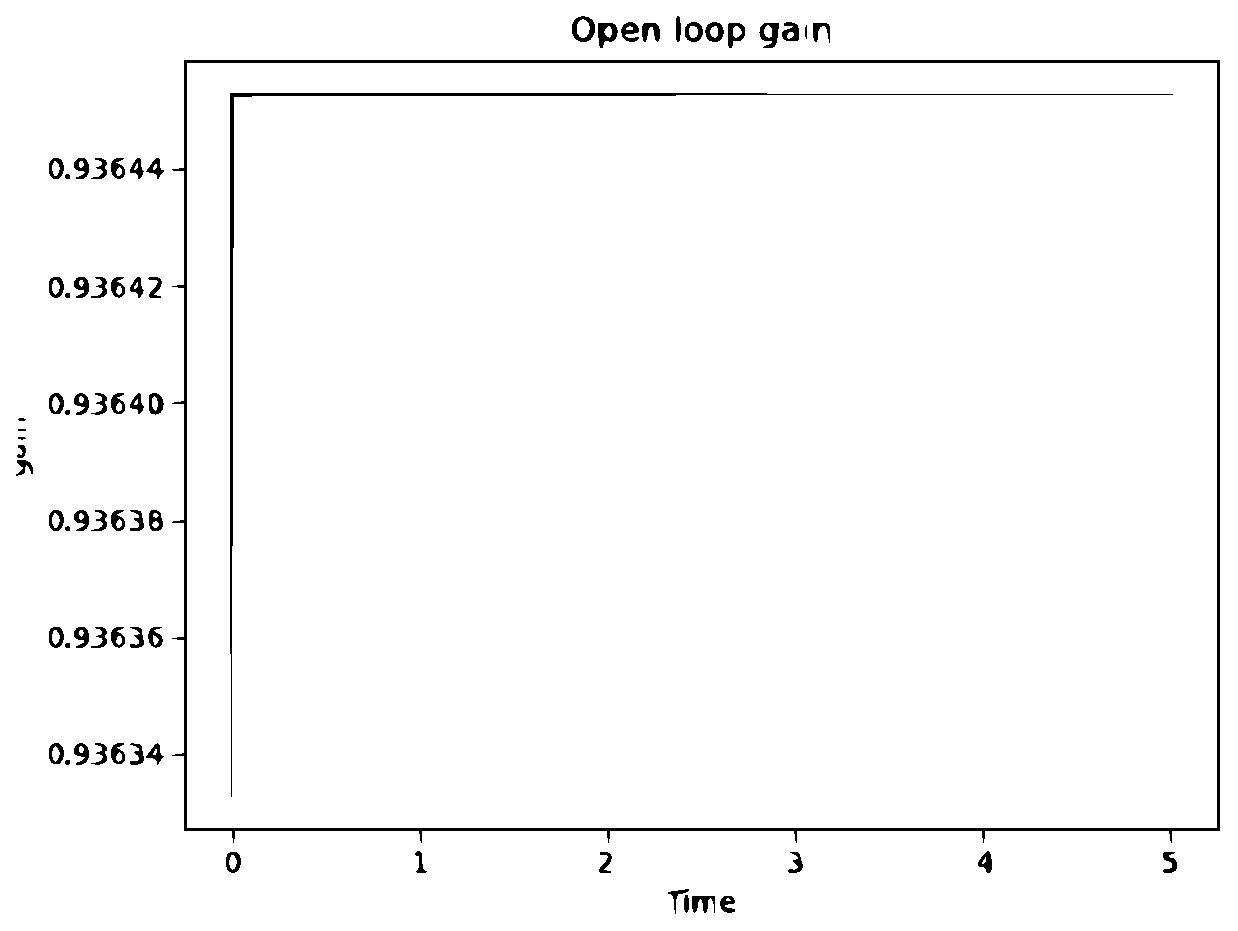
\includegraphics[width=\columnwidth]{./figs/es17btech11019/Gain}
\caption{}
\label{fig:ep18btech11016_feed_gain}
\end{figure}

\begin{figure}[!ht]
	\centering
    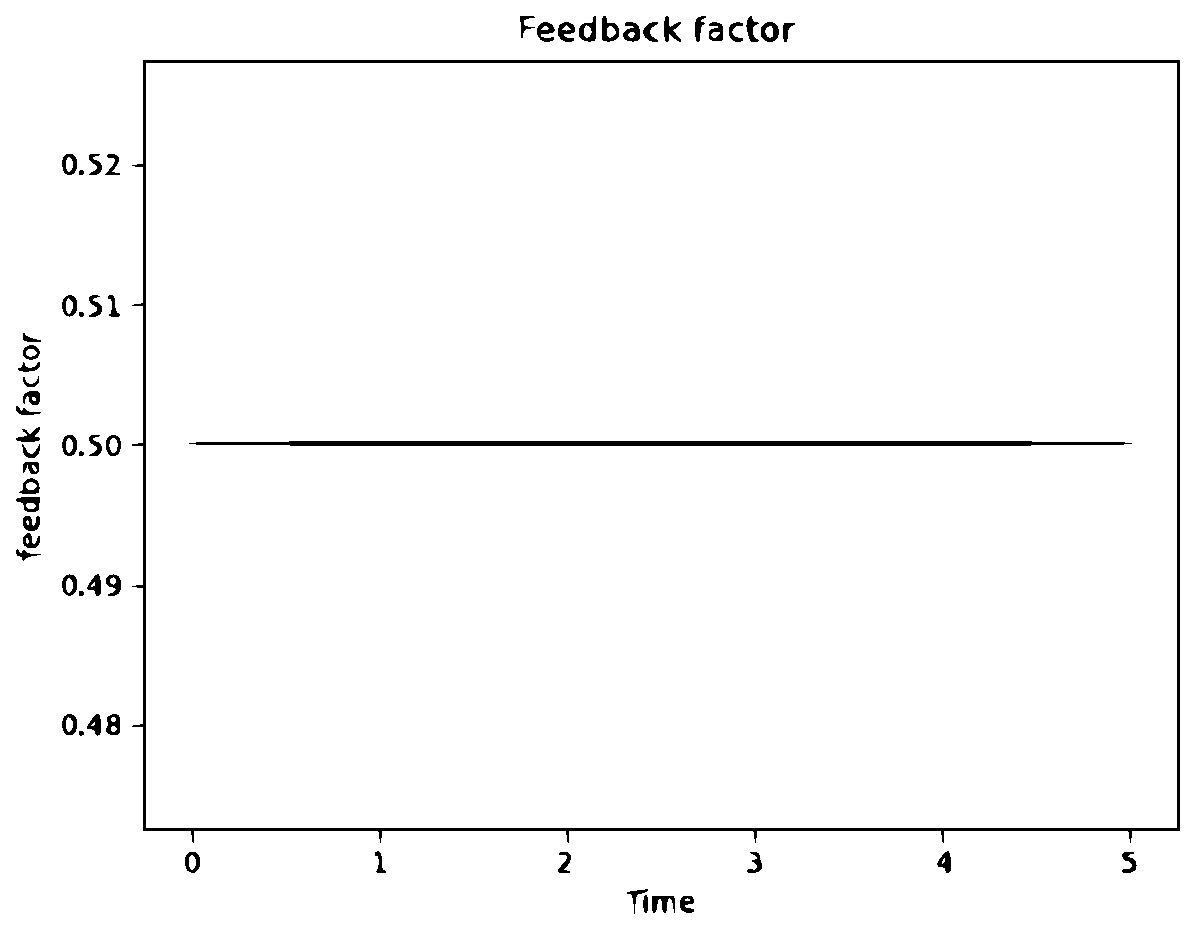
\includegraphics[width=\columnwidth]{./figs/es17btech11019/feedbackfactor}
\caption{}
\label{feedback factor}
\end{figure}
\renewcommand{\thefigure}{\theenumi}

Find the netlist of the simulated circuit here:
\begin{lstlisting}
    codes/es17btech11019/spice/es17btech11019.net
\end{lstlisting}

Python code used for generating the output:
\begin{lstlisting}
    codes/es17betch11019/spice/es17btech11019.py
\end{lstlisting}

\end{enumerate}